
\documentclass{article}

\usepackage{fontspec}
\usepackage{polyglossia}
\setdefaultlanguage{greek}
\setotherlanguage{english}
% Ορισμός βασικού font ως Noto Serif (βεβαιωθείτε ότι είναι εγκατεστημένο)
\setmainfont{Noto Serif}
% Ορισμός monospace font για την ορθή απόδοση ελληνικών χαρακτήρων στα \texttt{}
\newfontfamily\greekfonttt{Noto Sans Mono}

\usepackage{amsmath}
\usepackage{graphicx}
\usepackage{hyperref}
\title{Αναλυτική Αναφορά Ανάλυσης Δεδομένων ΑΕΠ}
\author{Θεόδωρος Κούρταλης}
\date{\today}
\begin{document}
\maketitle

\section{Εισαγωγή}
Η παρούσα αναφορά παρουσιάζει τη διαδικασία ανάλυσης των δεδομένων ΑΕΠ από το αρχείο \texttt{GDP\_data.mat}. Οι κύριες μεταβλητές είναι ο Ονομαστικός ΑΕΠ, ο Πραγματικός ΑΕΠ και ο Δείκτης ΑΕΠ. Από τον ονομαστικό και τον πραγματικό ΑΕΠ υπολογίστηκε ο GDP Deflator μέσω του τύπου:
\[
\text{GDP Deflator} = \frac{\text{Nominal GDP}}{\text{Real GDP}} \times 100.
\]
Εφαρμόστηκε ο φυσικός λογαρίθμος για τον υπολογισμό των ρυθμών ανάπτυξης (ως πρώτες διαφορές των λογαρίθμων) και επαληθεύτηκε η σχέση:
\[
\Delta \log(\text{Nominal GDP}) = \Delta \log(\text{Real GDP}) + \Delta \log(\text{GDP Deflator}),
\]
με μέγιστη απόλυτη διαφορά: \textbf{0.00000}. 

\section{Μεθοδολογία}
\begin{enumerate}
    \item \textbf{Φόρτωση Δεδομένων:} Τα δεδομένα εξήχθησαν από το αρχείο \texttt{GDP\_data.mat} χρησιμοποιώντας το \texttt{scipy.io.loadmat}. Οι βασικές σειρές είναι:
    \begin{itemize}
       \item \texttt{nominal\_gdp} --- Ονομαστικός ΑΕΠ.
       \item \texttt{real\_gdp} --- Πραγματικός ΑΕΠ.
       \item \texttt{gdp\_index} --- Δείκτης ΑΕΠ.
    \end{itemize}
    \item \textbf{Υπολογισμός GDP Deflator:} Ο GDP Deflator υπολογίστηκε ως:
    \[
    \text{GDP Deflator} = \frac{\text{Nominal GDP}}{\text{Real GDP}} \times 100.
    \]
    \item \textbf{Λογαριθμικός Μετασχηματισμός και Υπολογισμός Ρυθμών Ανάπτυξης:} Εφαρμόστηκαν οι φυσικοί λογαρίθμοι στις σειρές και στη συνέχεια υπολογίστηκαν οι ρυθμοί ανάπτυξης ως οι πρώτες διαφορές των λογαρίθμων.
    \item \textbf{Εύρεση Βάσης (Base Year):} Η βάση ορίζεται ως η χρονική περίοδος κατά την οποία ο ονομαστικός ΑΕΠ είναι ίσος (ή όσο το δυνατόν πιο κοντά) στον πραγματικό ΑΕΠ. Για την Ευρωζώνη η βάση βρίσκεται στο index \textbf{20}, και για την Ελλάδα στο index \textbf{20}.
    
    \textit{Παρατήρηση:} Και οι σειρές του ονομαστικού και του πραγματικού ΑΕΠ παρουσιάζουν τάση (κλίση), οπότε η εύρεση της βάσης προσφέρει ένα σημείο αναφοράς για τη σύγκριση των μεταβολών.
    
    \item \textbf{Σχεδίαση Γραφημάτων:} Για κάθε χώρα δημιουργήθηκαν:
    \begin{itemize}
        \item Γράφημα υπο-διαγραμμάτων (3 υπογράμματα) που απεικονίζουν τους ρυθμούς ανάπτυξης.
        \item Ένα ενιαίο γράφημα (side by side) που συγκρίνει τους ρυθμούς ανάπτυξης μεταξύ της Ευρωζώνης και της Ελλάδας.
    \end{itemize}
\end{enumerate}

\section{Αποτελέσματα}
Το ενιαίο γράφημα που συγκρίνει τους ρυθμούς ανάπτυξης για τις δύο χώρες παρουσιάζεται στην εικόνα:
\begin{figure}[h!]
    \centering
    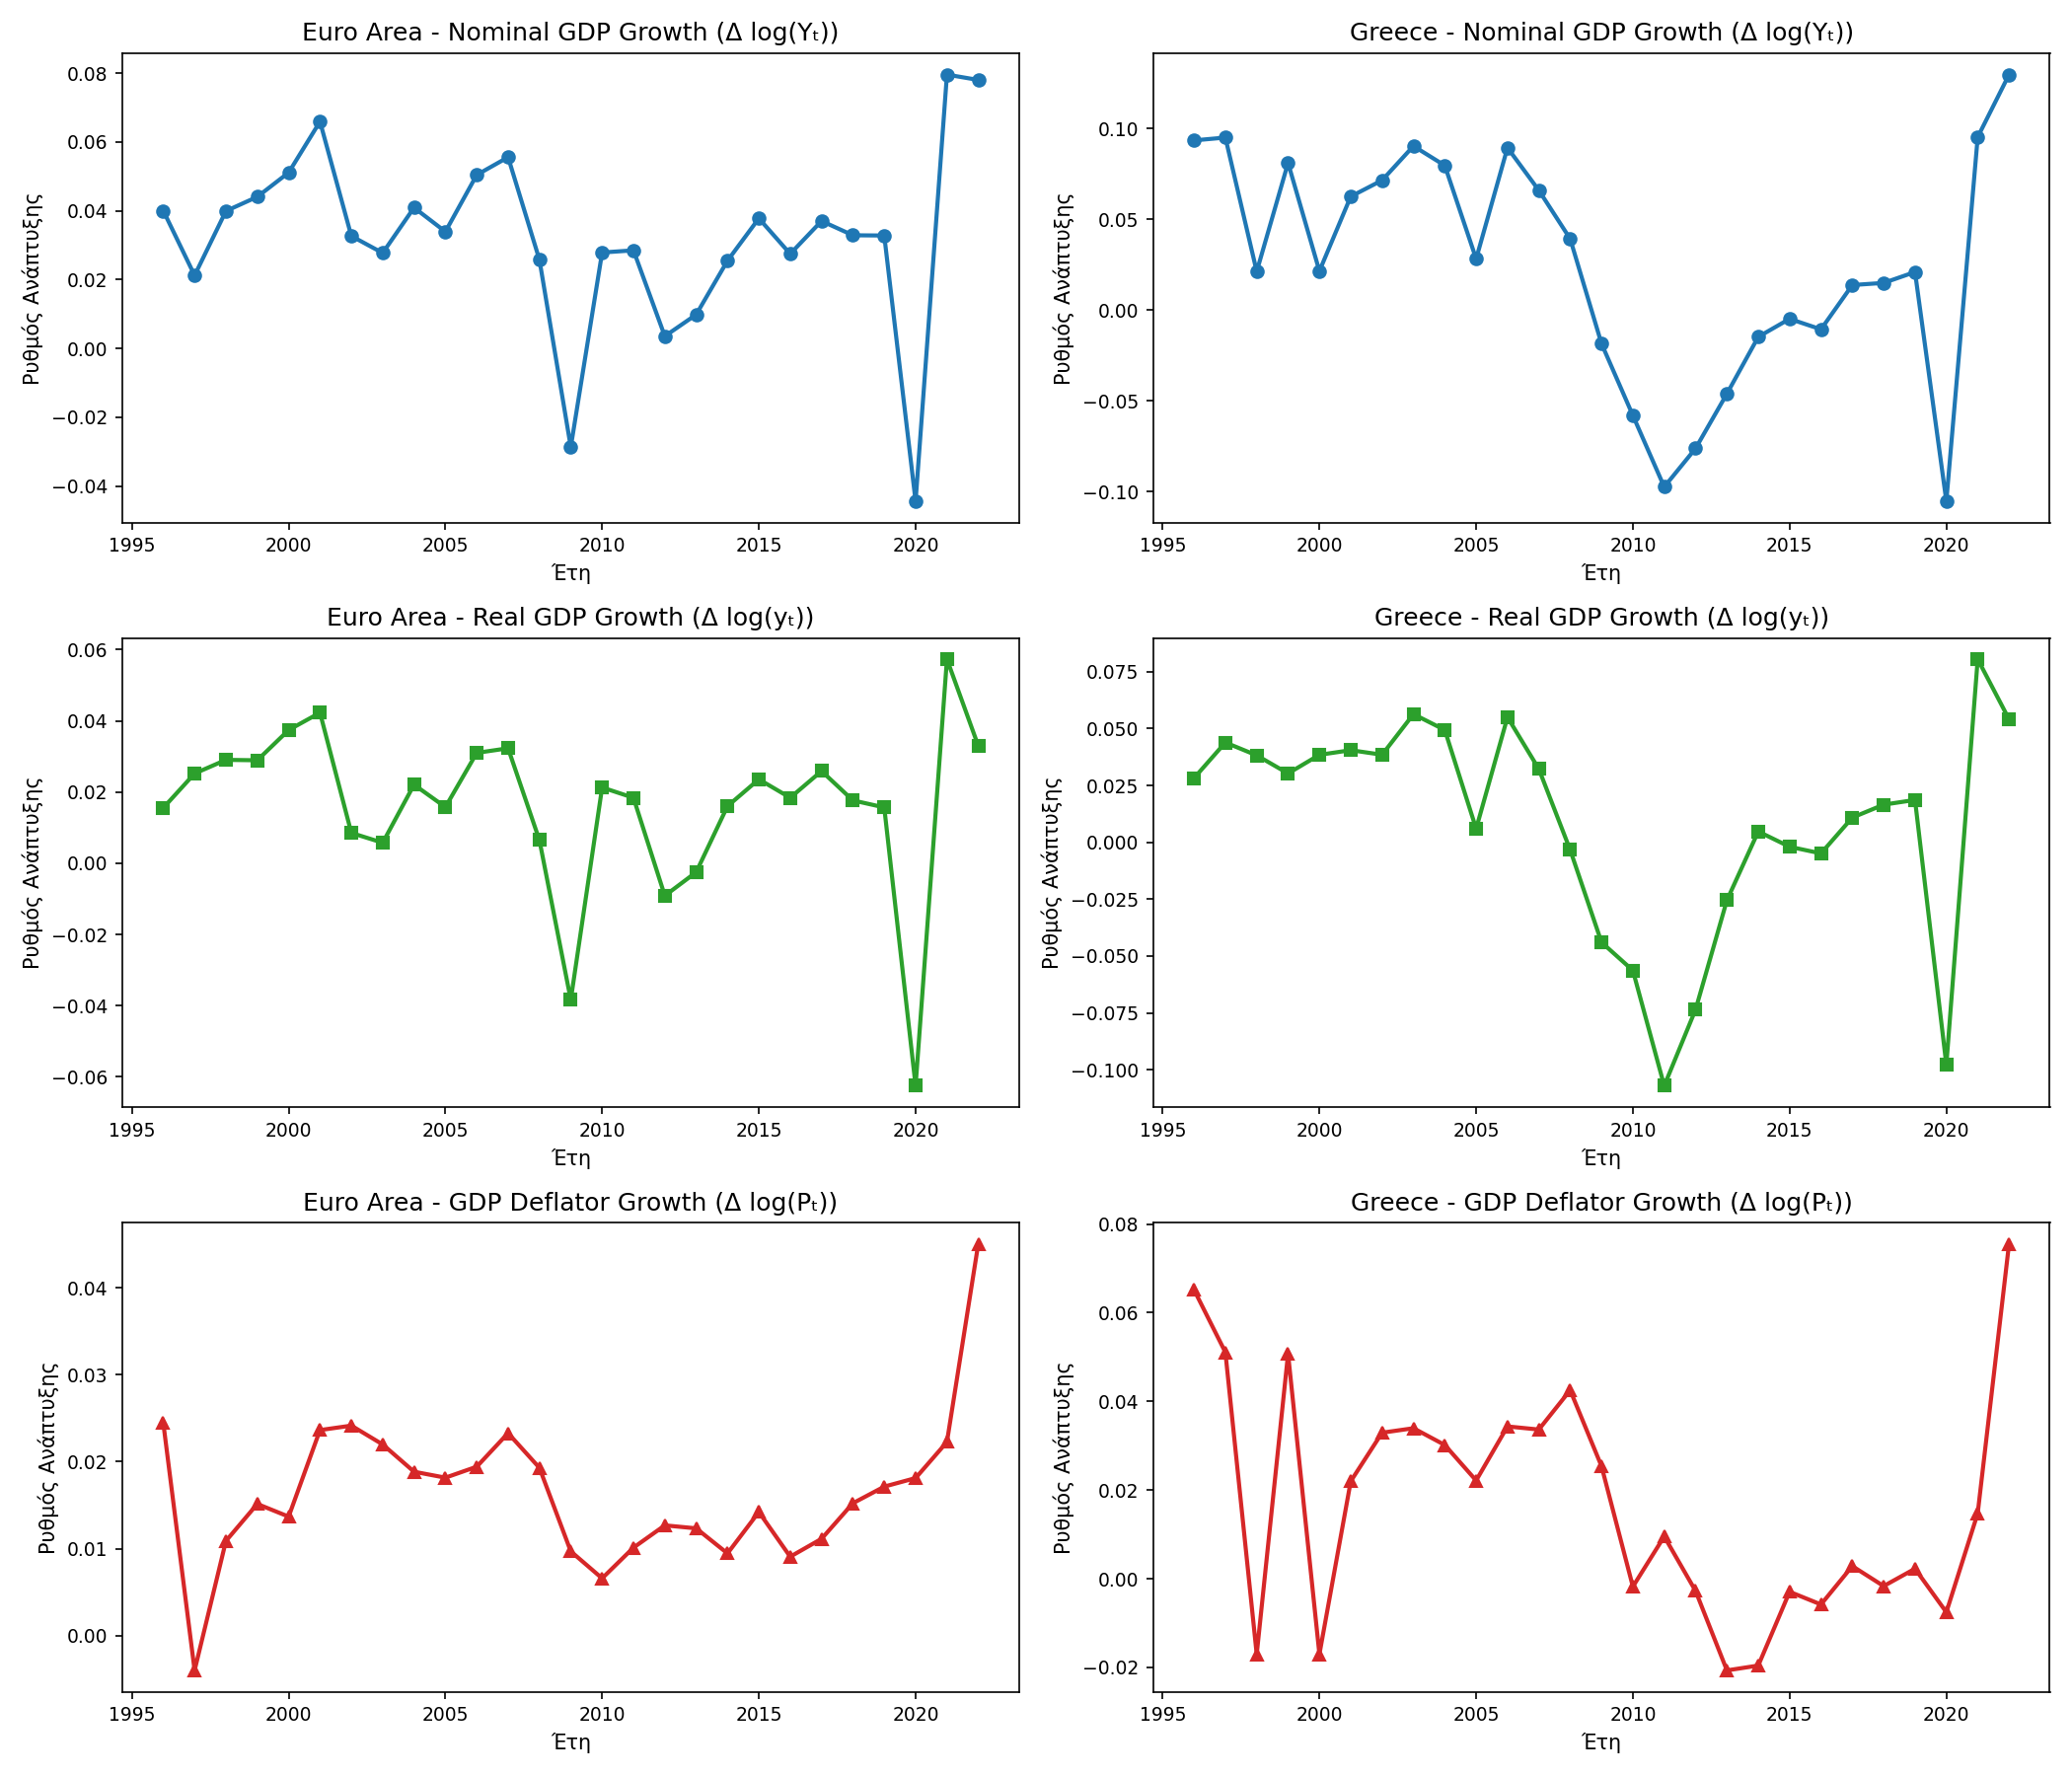
\includegraphics[width=0.9\textwidth]{side_by_side_growth.png}
    \caption{Σύνοψη ρυθμών ανάπτυξης για την Ευρωζώνη και για την Ελλάδα. Τα δεδομένα αναπαριστούν τα έτη από 1996 έως 2022.}
\end{figure}

Τα γραφήματα υπο-διαγραμμάτων για κάθε χώρα αποθηκεύτηκαν στα αρχεία:
\begin{itemize}
    \item \texttt{subplots\_euro\_area.png} για την Ευρωζώνη.
    \item \texttt{subplots\_greece.png} για την Ελλάδα.
\end{itemize}


\end{document}
    